\clearpage
\section{Description and Data Analysis}

We started by measuring the resonance frequency of three different linear oscillating circuits.

\subsection{Linear Oscillating Circuits}

\subsubsection{Circuit 1}

Before using the resistors, we measured their resistance $R_1$ with the digital multimeter. Also did we measure the resistance of the inductor $R_L$. For the values of the inductance $L$ and the capacitance $C$, we took the values written on the respective parts.

\begin{tabular}{l l l}
Components used & $R_1 = (15.0 \pm 0.1)\ \Omega$ & \\
 & $L=3.5\ H$ & $R_L = (102.3 \pm 0.1)\ \Omega$\\
 & $C=100\ nF$ & \\
\end{tabular}

For the total resistance follows $R = R_1 + R_L = 117.3 \Omega$ with the error $s_R = \sqrt{s_{R_1}^2 + s_{R_L}^2} = 0.14$ 
So, the theoretical resonance frequency results from:

$$f_{res,theo} = \frac{1}{2\pi}\sqrt{\frac{1}{LC}-\frac{R^2}{4L^2}} = 269.0\ Hz$$

with the error:

$$s_f = \frac{Rs_R}{16\pi^2fL^2} = 2.8\cdot 10^{-5}\ Hz$$

We then started by measuring the amplitude $A$ for different frequencies near the resonance frequency, in order to find the exact resonance frequency. We plotted the amplitude $A$ against the frequency and obtained:

\begin{figure}[H]
\centering 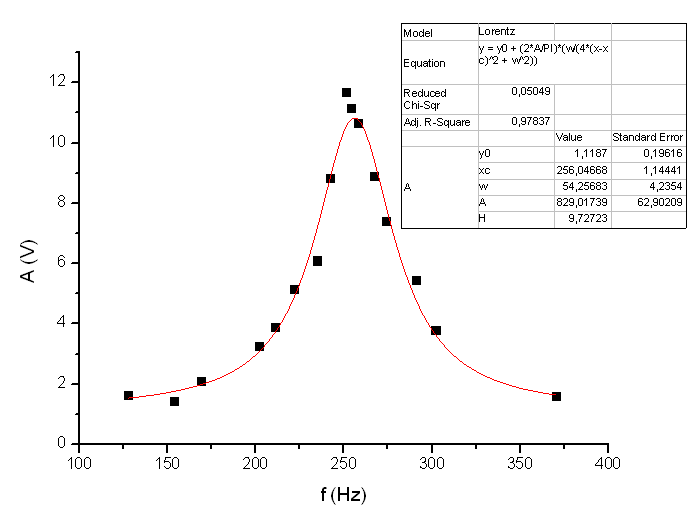
\includegraphics[width=0.9\textwidth]{Bilder/1a.png}
\caption{Circuit 1}
\end{figure}

We estimated a relative error of about 2\% for the driving voltage and frequency. We used a Lorentz-Peak to fit the data, which is defined by 

$$ A = y_0 + \frac{2Aw/\pi}{4(x-x_c)^2 + w^2} $$

In our case the constant offset $y_0$ should be $y_0 = 0V$ or very close to that. It is 1.12 V, which is close enough. From the location of the maximum of the Lorentz distribution we obtain the resonance frequency of the system:

$$\boxed{f_{res} = x_c = (256.05 \pm 1.14)\ Hz}$$

The theoretical value lies within 12 errors of this value and deviates by 5\%.

\subsubsection{Circuit 2}

\begin{tabular}{l l l}
Components used& $R_1 = (15.0 \pm 0.1)\ \Omega$ & \\
 & $L=69.6\ mH$ & $R_L = (4.1 \pm 0.1)\ \Omega$\\
 & $C=1\ \mu F$ & \\
\end{tabular}

$\Rightarrow R = (19.1 \pm 0.1)\ \Omega$

$\Rightarrow f_{res,theo} = (603.03 \pm 0.01)\ Hz$

Again did we measure the behavior of the amplitude by changing the frequency near $f_{res,theo}$. We used a Lorentz-Peak to fit the data: 

\begin{figure}[H]
\centering 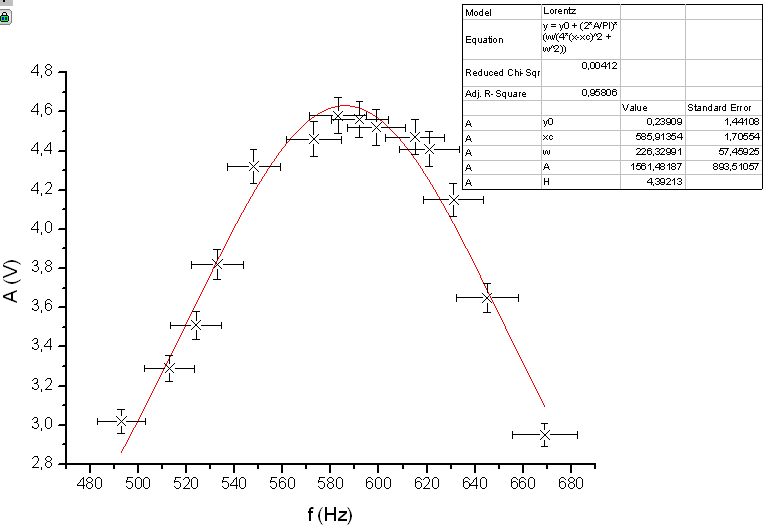
\includegraphics[width=0.9\textwidth]{Bilder/1b.png}
\caption{Circuit 2}
\end{figure}

$y_0 = (0.24 \pm 1.44)\ V$, which we can consider as being zero. The resonance frequency resulting from the peak is: 

$$\boxed{ f_{res} = x_c = (585.91 \pm 1.71)\ Hz}$$

This theoretical value lies within 11 standard deviations of this value and deviates by 3\%.


\subsubsection{Circuit 3}

\begin{tabular}{l l l}
Components used & $R_1 = (51.0 \pm 0.1)\ \Omega$ & \\
 & $L=20.1\ mH$ & $R_L = (1.2 \pm 0.1)\ \Omega$\\
 & $C=10\ nF$ & \\
\end{tabular}

$\Rightarrow R = (52.2 \pm 0.1)\ \Omega$

$\Rightarrow f_{res,theo} = (11224.02 \pm 0.01)\ Hz$

The Lorentz-Fit of the data near the theoretical resonance frequency looks like this:

\begin{figure}[H]
\centering 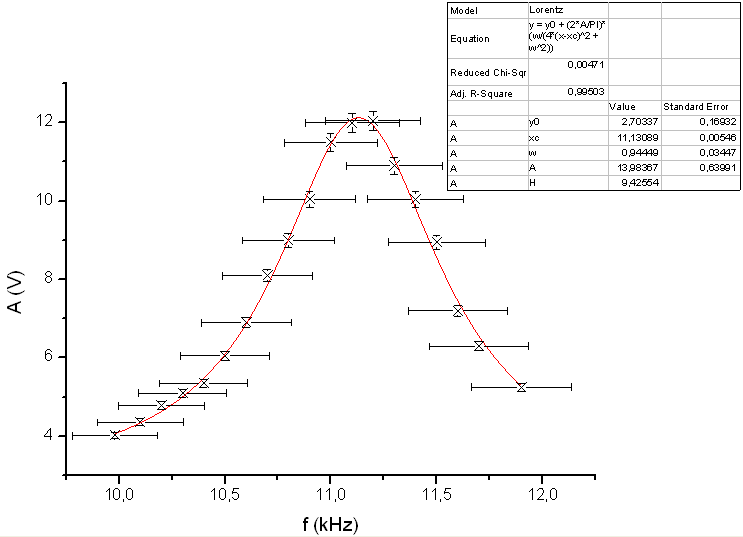
\includegraphics[width=0.9\textwidth]{Bilder/1c.png}
\caption{Circuit 3}
\end{figure}

The offset is as follows: $y_0 = (2.70 \pm 0.17)\ V$, which is quite far off from zero (16 standard deviations). For the resonance frequency, we get:

$$\boxed{ f_{res} = x_c = ( 11130.89 \pm 5.46)\ Hz}$$

So, the calculated value for the resonance frequency lies within the 17th error of this value, and deviates by 0.8\%.

\paragraph{Error Discussion}

Even though our fitted values for the resonance frequencies lie very close to the calculated values, i.e. under 5\%, the theoretical frequencies all lie within the 11th or 12th standard deviation. We conclude therefore, that the error calculated by the fit is too small to be used as a factor to determine how good our measurements were.

\subsection{Nonlinear Oscillating Circuit}

For the nonlinear oscillating circuit, we had a lot of trouble finding a diode, for which we could actually see the resonance frequency by changing the input frequency. We finally took the diode called \emph{1N4007}, and we assumed by testing, that the resonance frequency should be about 155 kHz. We then measured the Amplitude of the circuit while changing the frequency of the input sine-sunction to find the exact resonance frequency. The amplitude of the sine-function was set to minimum, in order to prevent chaotic behavior.

In addition to the diode, we embedded a resistor ($R_1= 0.2 \ \Omega$) and an inductor ($L=10\ mH$ and $R_L = 50.0\ \Omega$) into the circuit. The resulting resistance is: $R = (50.2 \pm 0.1)\ \Omega$. We used a Lorentz-Fit to find the resonance frequency:

\begin{figure}[H]
\centering 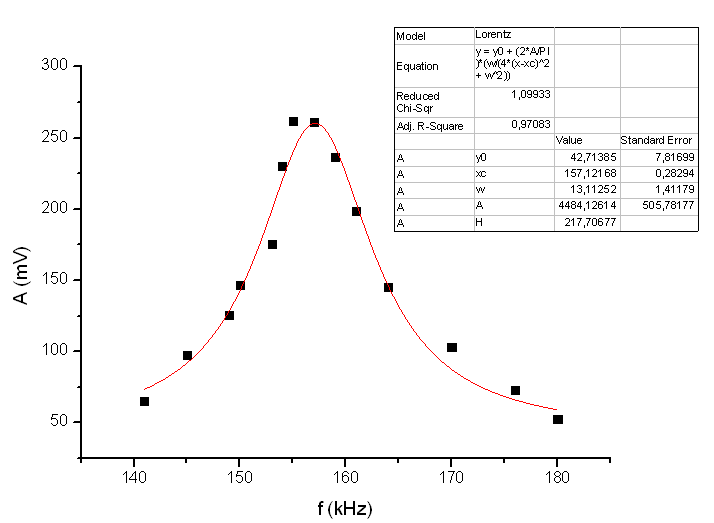
\includegraphics[width=\textwidth]{Bilder/fresnl.png}
\caption{Determination of the resonance frequency}
\end{figure}

Therewith it is:

$$f_{res}=(157.1 \pm 13.1)\ kHz$$

This resonance frequency is by far larger than the ones on the linear oscillating circuits. Those were in the lower two-digit kilohertz region or even smaller then 1 kHz, while the nonlinear oscillating circuit resonance frequency surpasses 100 kHz.\\
We then continued our measurements with a fixed frequency of $f = 156 kHz$.
We gradually changed the amplitude of the frequency generator to analyze the behavior on the oscilloscope. Firstly, we were able to see a second sine-function with a smaller amplitude overlaying the first one. We interpreted this behavior as the first bifurcation of the nonlinear system. By choosing a greater time resolution we saw an odd behavior on a larger scale. We obtained a non-sinusoidal-function, but which was still periodic (see figure \ref{aaa}).

\begin{figure}[H]
\begin{minipage}{0.5\textwidth}
\centering 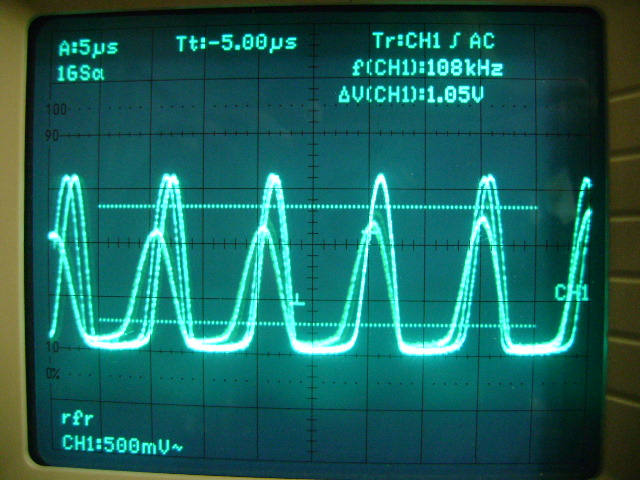
\includegraphics[width=\textwidth]{Fotos/01.JPG}
\caption{First bifurcation}
\end{minipage}
\begin{minipage}{0.5\textwidth}
\centering 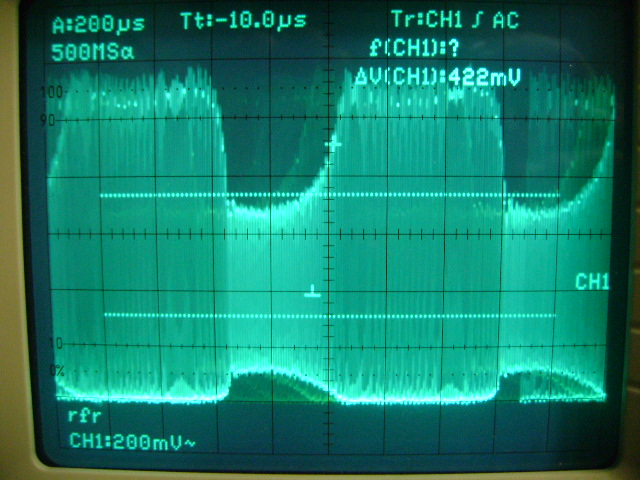
\includegraphics[width=\textwidth]{Fotos/02.JPG}
\caption{Greater time resolution}
\label{aaa}
\end{minipage}
\end{figure}

By continuing to turn up the amplitude, the sine-function started flickering, but we were sometimes able to see that more and more sine functions overlayed each other. After several tries, we succeeded to make a decent picture representing this muliple overlay:

\begin{figure}[H]
\centering 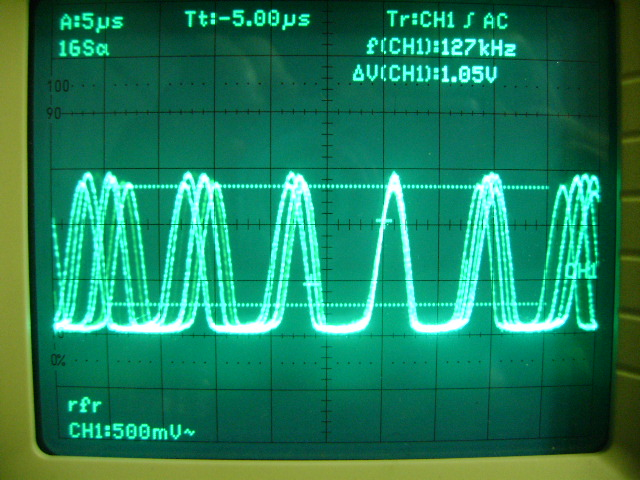
\includegraphics[width=0.5\textwidth]{Fotos/03.JPG}
\caption{More overlaying sine-functions}
\end{figure}

Finally, we tried to set up the Feigenbaum-diagram of our chaotic system. In order to do this, we switched to x-y-diagram of the oscilloscope, where we plotted the frequency generator amplitude against the tension of the diode. We adjusted the frequency, until we could see the bifurcation diagram. We obtained the following picture:

\begin{figure}[H]
\centering 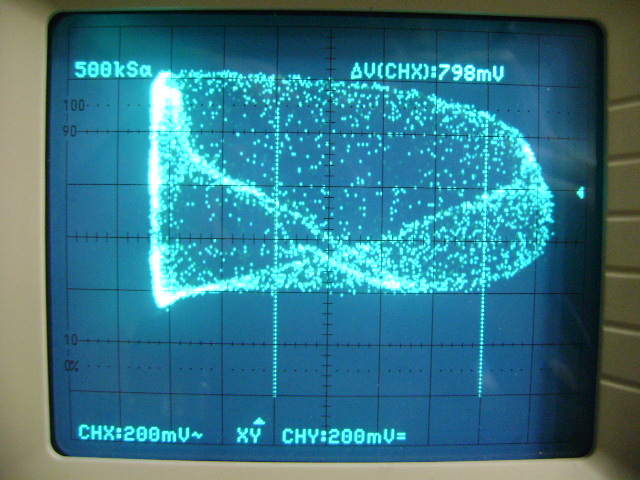
\includegraphics[width= 0.7\textwidth]{Fotos/04.JPG}
\caption{x-y-plot on oscilloscope}
\end{figure}

It was very hard to be able to read the amplitude of the third bifurcation, but since it was the only diode, for which we could find any resonance frequency at all, we tried to measure it. By changing the amplitude of the function generator's signal, we measured the resulting changes of the different tensions we saw on the x-y-plot on the oscilloscope. We then plotted the tension of the function generator against those on the diode and obtained a Feigenbaum-diagram, which unfortunately doesn't represent what we expected at all. It is possible to see the first bifurcation, but after that, we cannot use it to make any kind of statement considering the Feigenbaum-constants or the other bifurcations. In retrospect we believe, that might have started our observations at an amplitude that was already driving the system into chaos. The bifurcations we observed would then correspond to bifurcations within periodic windows.

So, we redid the whole measurements together with our fellow students\footnote{Christian Grumber and Yannick Linke} with the following parameters: $L = 9.5 mH$, $R_L=(0.8\pm 0.1)\Omega$, $R_1=(15.0 \pm 0.1) \Omega$ and with the diode \emph{1N4007}. It follows, that $R = (15.8 \pm 0.1) \Omega$.

The x-y-plot looked like this:

\begin{figure}[H]
\centering 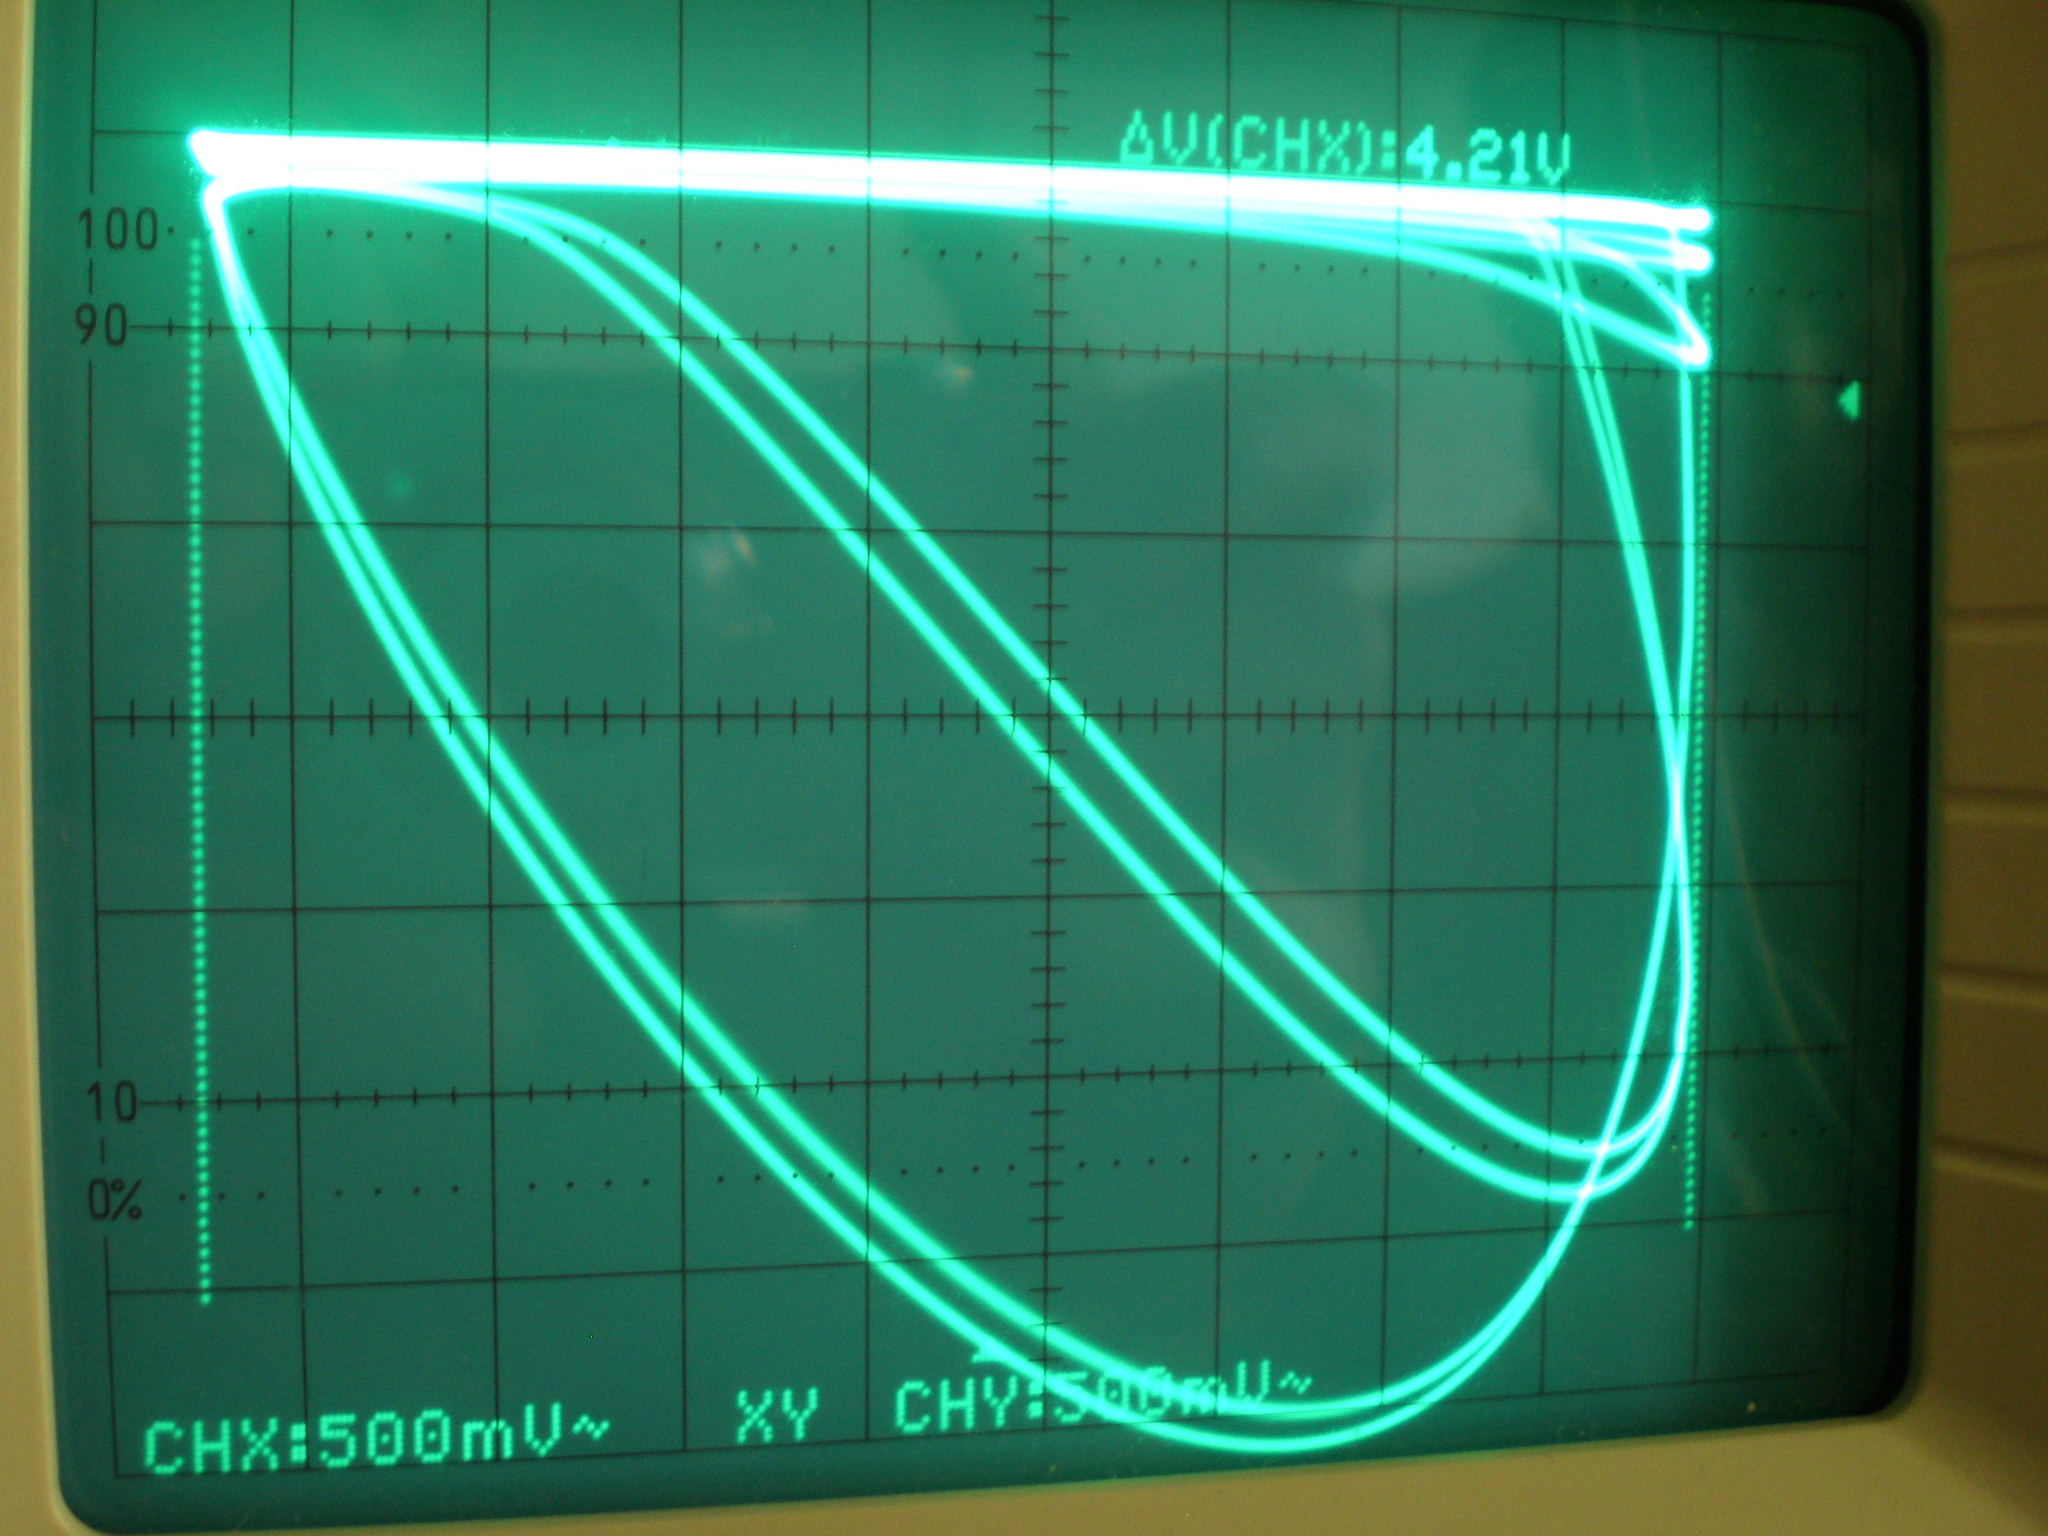
\includegraphics[width= 0.6\textwidth]{Fotos2/01.JPG}
\caption{second x-y-plot on oscilloscope}
\end{figure}

By changing the amplitude and measuring the resulting voltages we were able to make a new bifurcation diagram, which looks like this:

\begin{figure}[H]
\centering 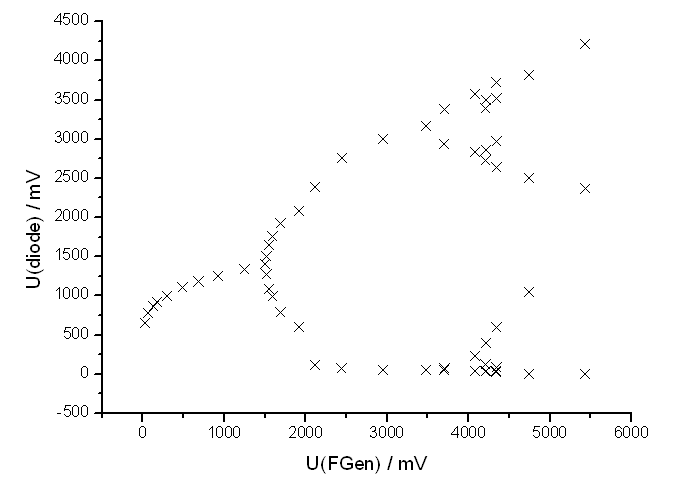
\includegraphics[width= 0.95\textwidth]{Bilder/bifdiag.png}
\caption{Bifurcation Diagram}
\end{figure}

Beginning from 4340 mV, we started seeing chaotic behavior. The voltage on the diode wasn't discrete anymore but started being continuous between the branches of the diagram. In this diagram, one can see 3 bifurcation which makes is usable to interpret and calculate the Feigenbaum-Constants. The three first bifurcation are located as follows:

\begin{center}
\begin{tabular}{c c}
n & $U_n / mV$\\ \hline
1 & $1520 \pm 10$\\
2 & $3700 \pm 10$\\
3 & $4210 \pm 10$
\end{tabular}
\end{center}

We can approximate the Feigenbaum-Constant $\delta$ by calculating the first term of its sequence, which is:

$$\boxed{\delta_1 = \frac{U_2-U_1}{U_3-U_2} = 4.275 \pm 68.62}$$

The error was calculated through:

$$s_\delta = \sqrt{\frac{\partial \delta}{\partial U_1}s_{U_1}^2 + \frac{\partial \delta}{\partial U_2}s_{U_2}^2 + \frac{\partial \delta}{\partial U_3}s_{U_3}^2} 
= \frac{s_U}{U_3-U_2}\sqrt{(U_3-U_2)^2 + (U_3-U_1)^2 + (U_2-U_1)^2}$$

with $s_U = s_{U_1} = s_{U_2} = s_{U_3}$. We can not explain why it turned out so huge, but still can say that our value for $\delta$ lies quite near at the theoretical value, which is $\delta$=4.669. Our error is approx. 9\%.

\begin{figure}[H]
\begin{minipage}{0.4\textwidth}
For the second Feigenbaum-Constant $\alpha$, we measure the distance between the two first branches at the moment of bifurcation and calculate $\alpha$ through:
$$\alpha = \frac{|D_1|}{|D_2|}$$
We measured: $D_1 \approx (3000 \pm 100) mV$ and $D_2 \approx (750\pm 100) mV$ and calculated:
\end{minipage}
\begin{minipage}{0.6\textwidth}
\centering 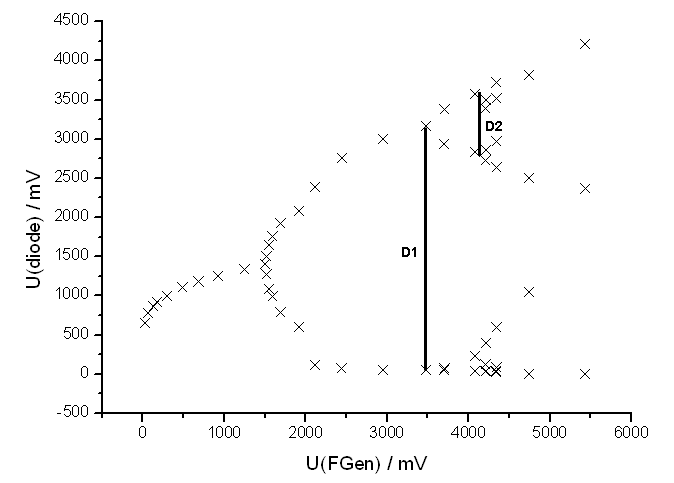
\includegraphics[width=\textwidth]{Bilder/bifdiagD.png}
\end{minipage}
\end{figure}

$$\boxed{\alpha = \frac{3000}{750} = 4.00 \pm 0.55}$$

So the theoretical value of $\alpha = 2.503$ lies within the third standard deviation of our experimental value.

In the last part of the experiment, we modulated the amplitude of the driving voltage with a triangular function (as well as other functions) and were thus able to see bifurcation diagrams in the x-y-plot function of the oscilloscope. We took photos of these bifurcation diagrams:

\begin{figure}[H]
\centering 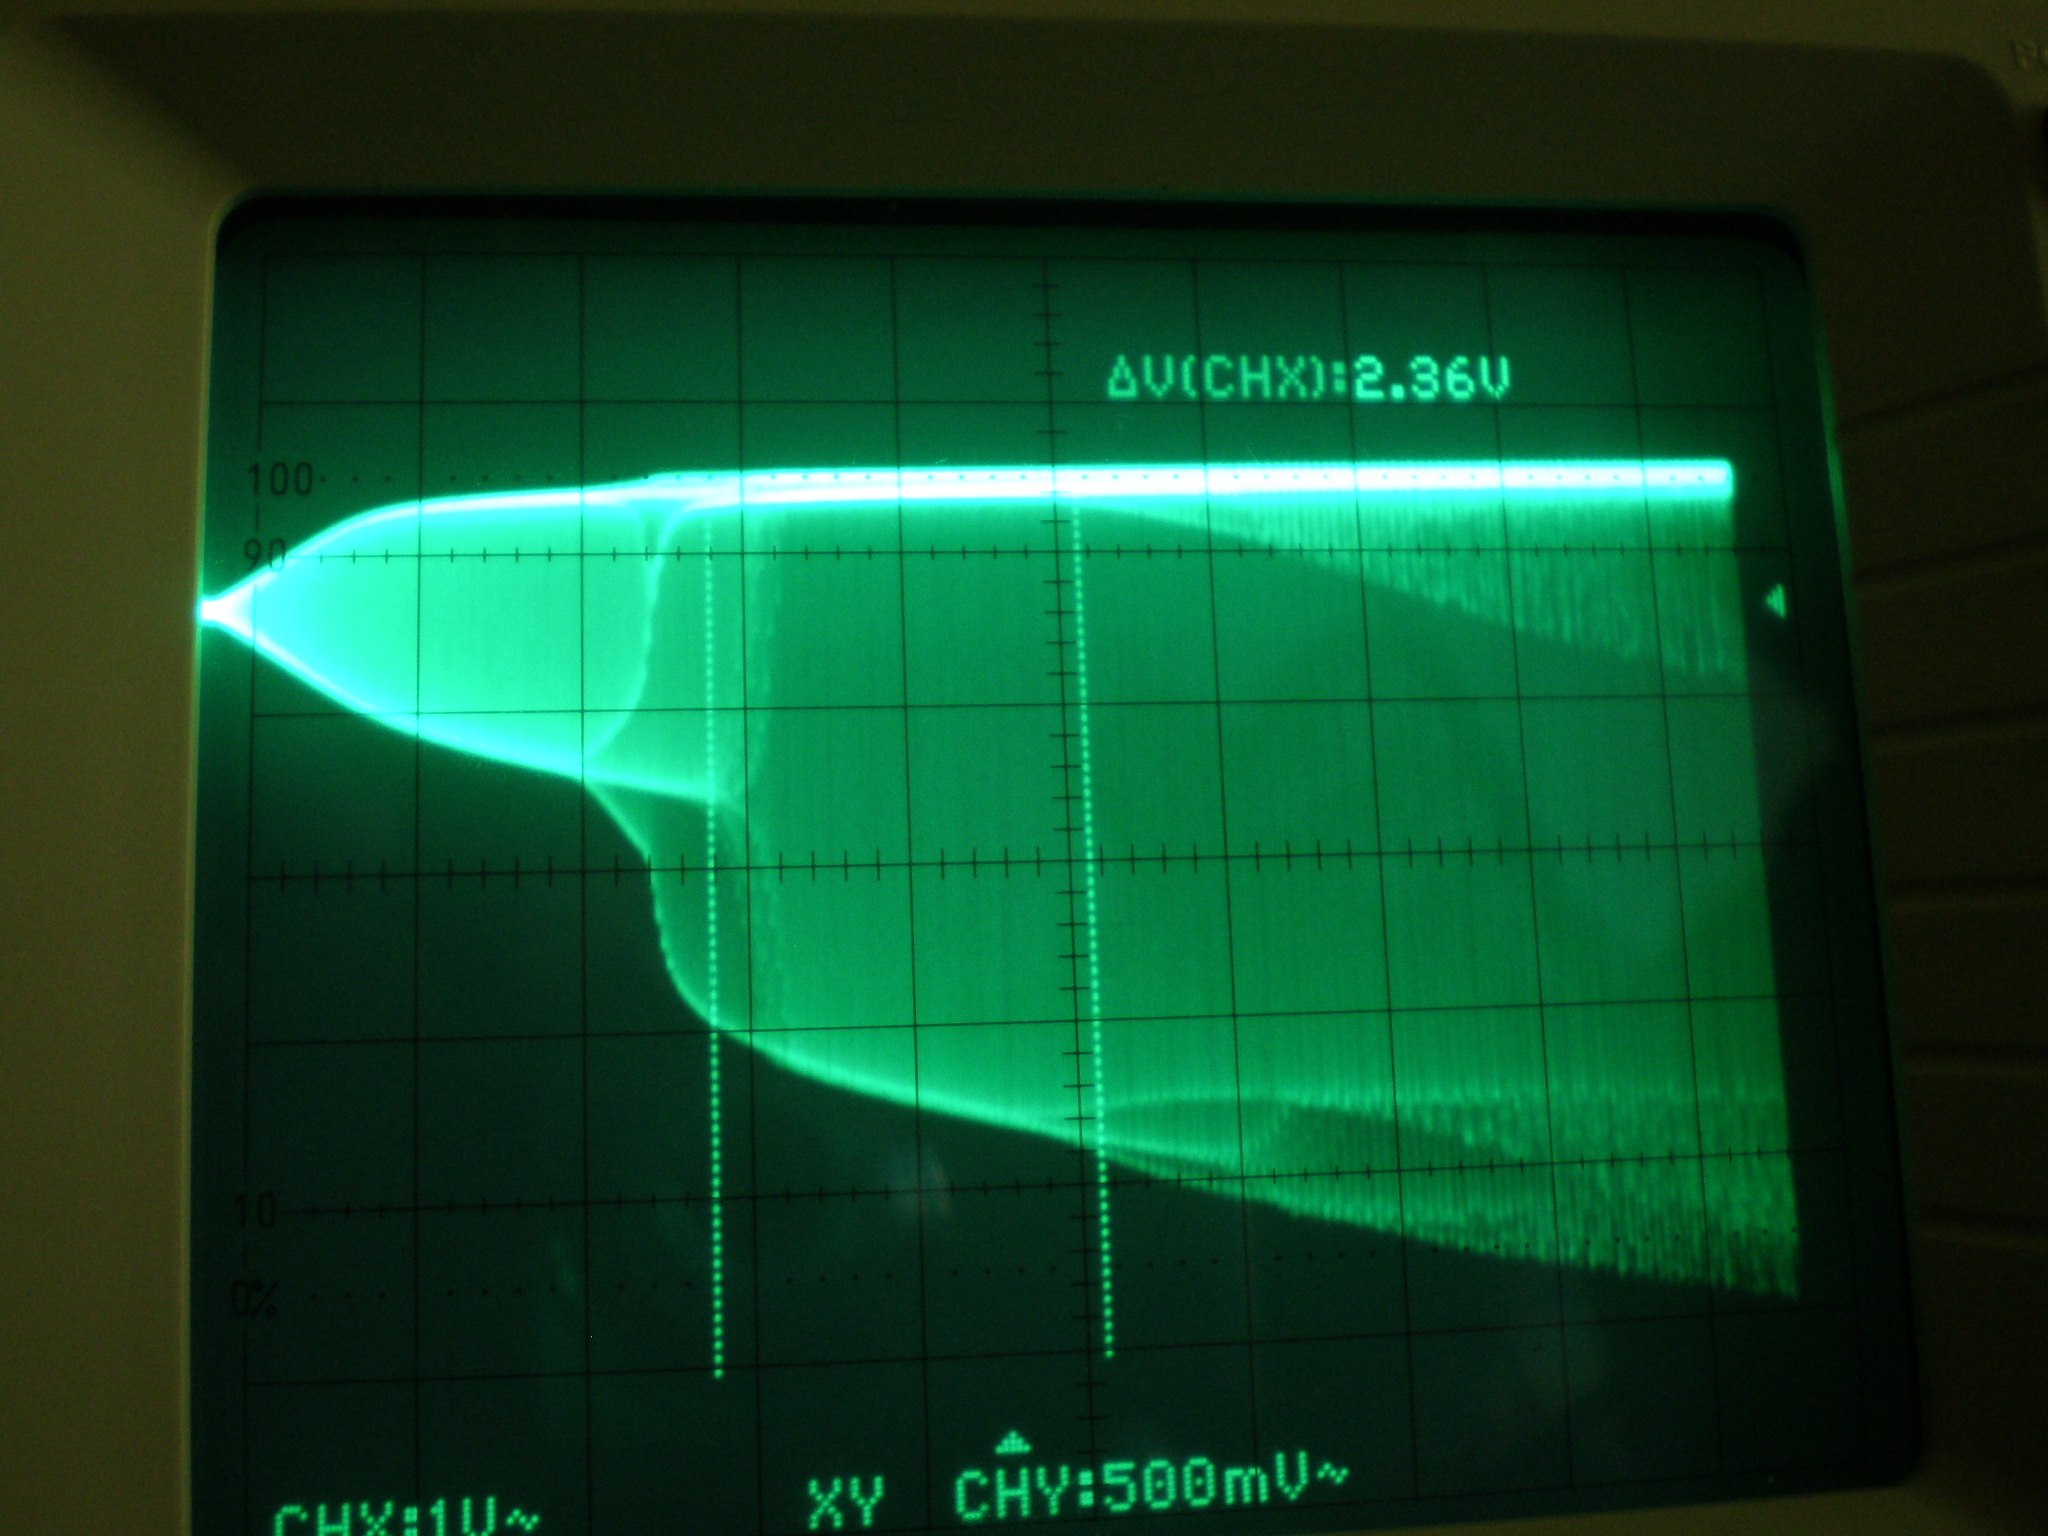
\includegraphics[width= 0.85\textwidth]{Fotos2/16.JPG}
\caption{Bifurcation Diagram with a triangular function}
\end{figure}

Other examples are:

\begin{figure}[H]
\begin{minipage}{0.5\textwidth}
\centering 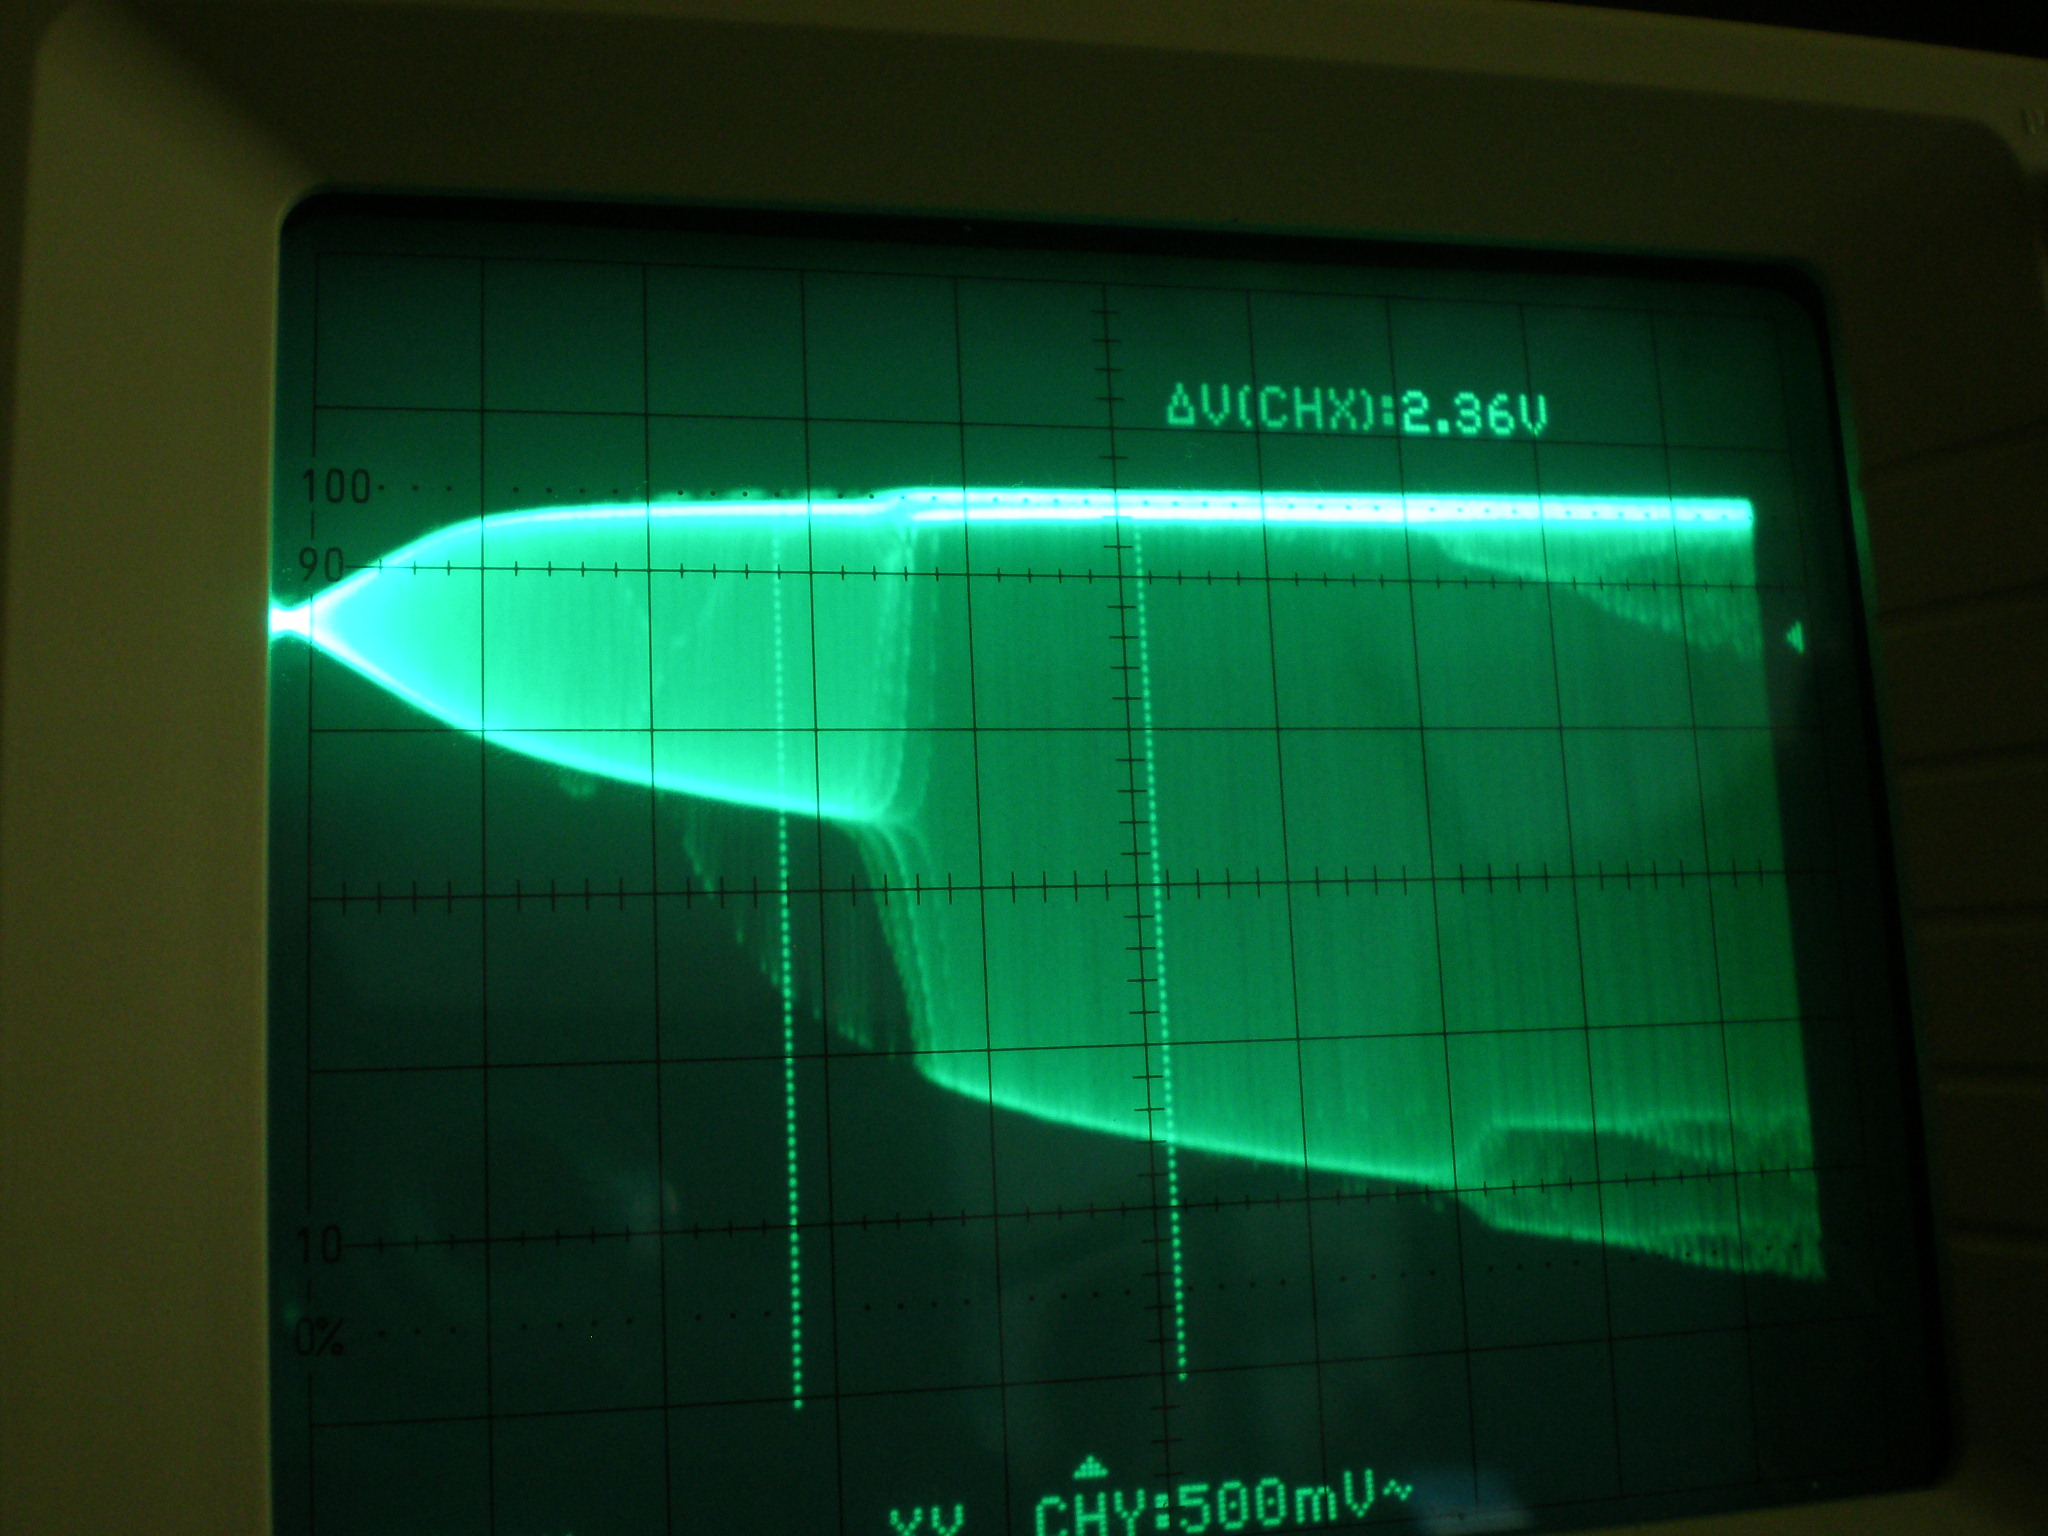
\includegraphics[width=\textwidth]{Fotos2/13.JPG}
\caption{Sawtooth}
\end{minipage}
\begin{minipage}{0.5\textwidth}
\centering 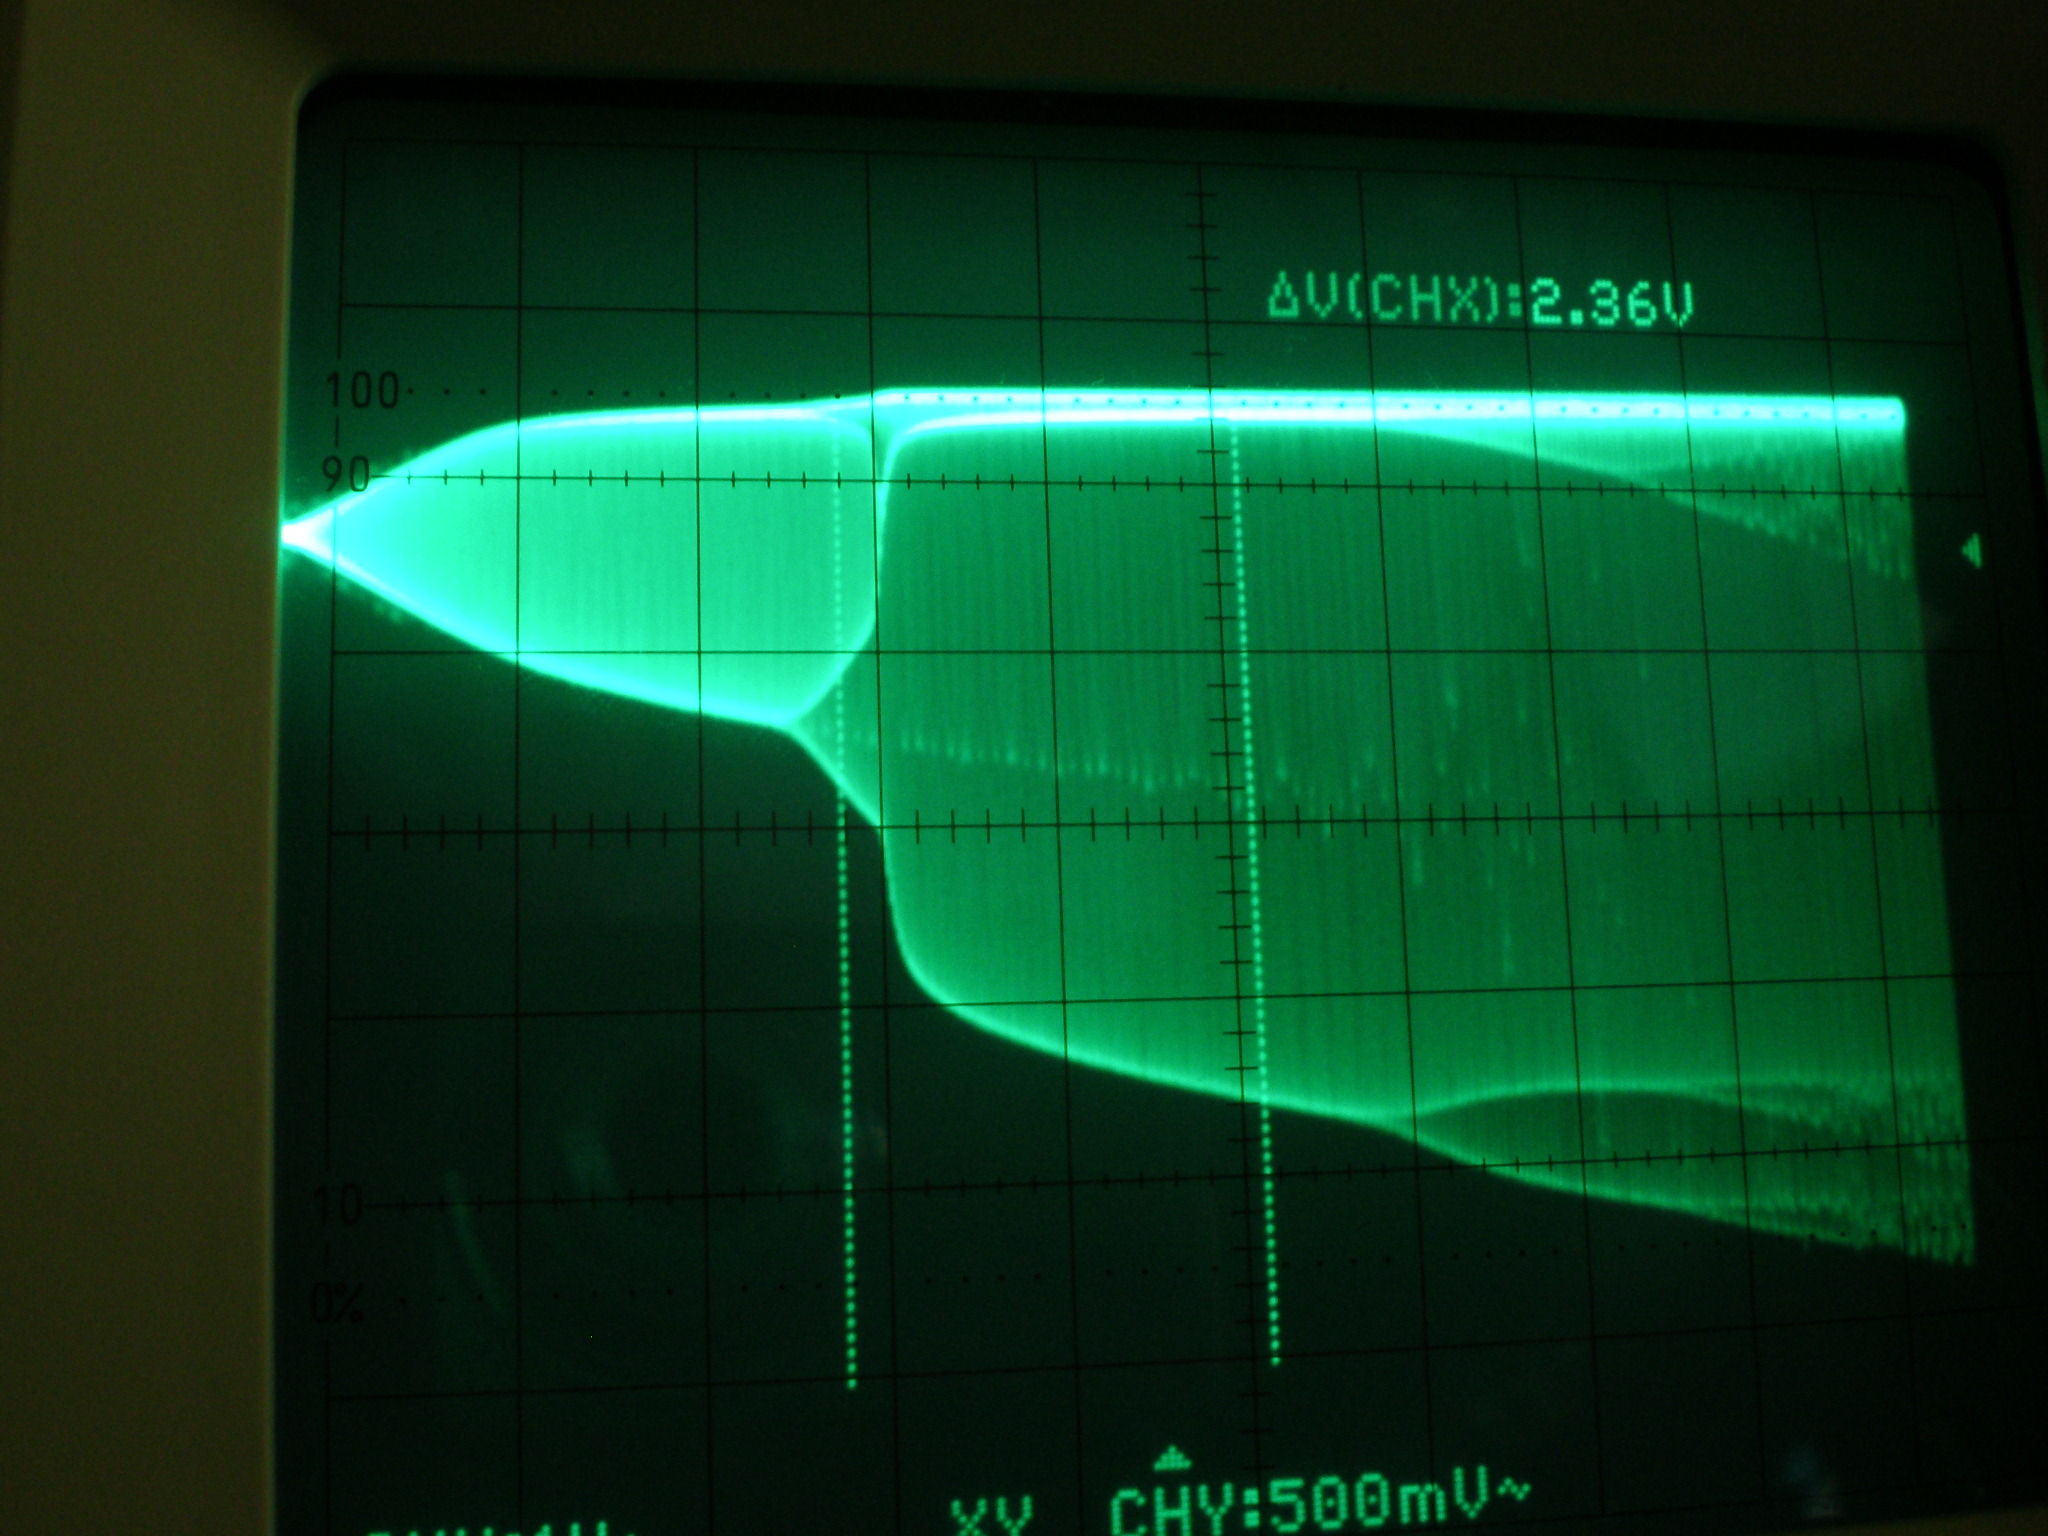
\includegraphics[width=\textwidth]{Fotos2/15.JPG}
\caption{Reverse Sawtooth}
\end{minipage}
\end{figure}

Here it is even possible to see hysteresis effects near the second bifurcation. Also did we try to modulate the sine function from the frequency generator with another sine function with lower frequency:

\begin{figure}[H]
\centering 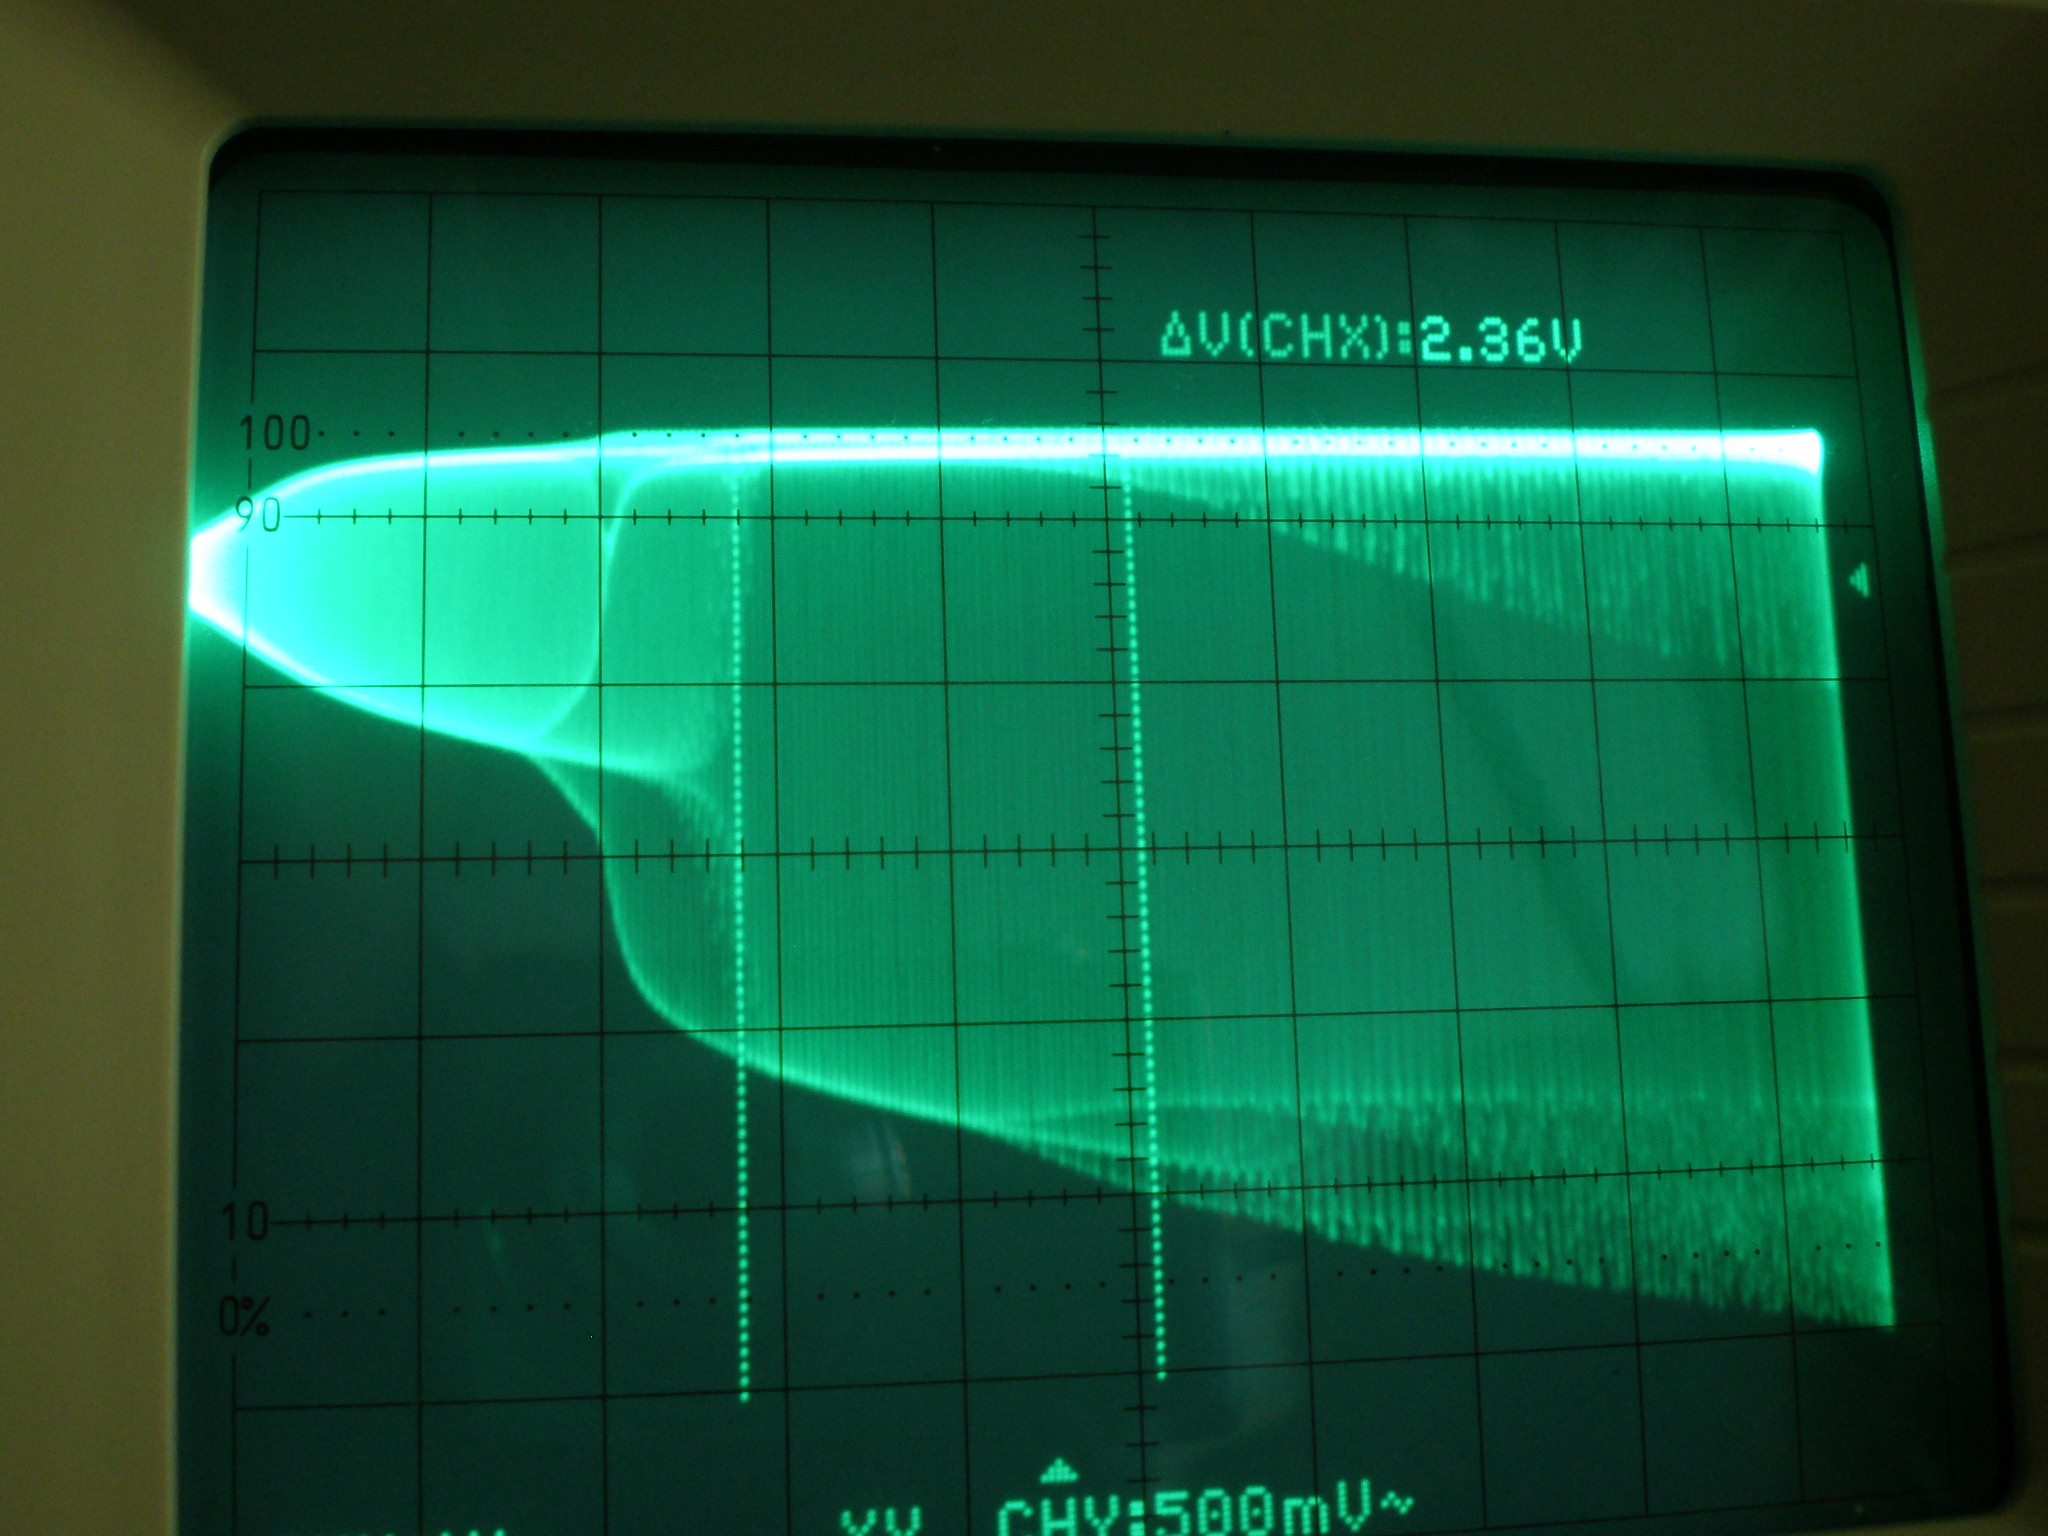
\includegraphics[width= 0.85\textwidth]{Fotos2/19.JPG}
\caption{Sine-function}
\end{figure}

